\section{Математическое описание}


\subsection{Алгебраические структуры}

 Множество $Z$ вместе с набором операций $\Sigma = \{\varphi_1, \ldots, \varphi_m\}$, $\varphi_i : Z^{n_i} \rightarrow Z$, где $n_i$ - арность операции $\varphi_i$, называется алгебраической структурой, универсальной алгеброй или просто алгеброй.


Коммутативное кольцо с единицей - алгебраическая структура $\langle Z; +, * \rangle$, которая обладает следующими свойствами:

\begin{enumerate}
  \item $(a + b) + c = a + (b + c)$ (сложение ассоциативно)
  \item $\exists \, 0 \in Z \; (\forall a \in Z : a + 0 = 0 + a = a)$ (существует нуль)
  \item $\forall a \in Z \; \exists (-a) \in Z : a + (-a) = 0$ (существует обратный элемент)
  \item $a + b = b + a$ (сложение коммутативно)
  \item $(a * b) * c = a * (b * c)$ (умножение ассоциативно)
  \item $a * (b + c) = a * b + a * c$ (умножение дистрибутивно относительно сложения)
  \item $a * b = b * a$ (умножение коммутативно)
  \item $\exists 1 \in Z \; (\forall a \in Z : a * 1 = 1 * a = a)$ (существует единица)
\end{enumerate}

«Малая» конечная арифметика - это коммутативное кольцо с единицей $\langle Z_{8}; +, * \rangle$, элементы которого являются одноразрядными символами. В данной работе используется множество $Z_{8} = \{a, b, c, d, e, f, g, h\}$.

«Большая» конечная арифметика - это коммутативное кольцо с единицей $\langle Z_8^n; +, * \rangle$, элементами которого являются слова длины \(n\), составленные из элементов
множества \(Z_8\), в котором операции сложения и умножения выполняются позиционно с
учётом переносов. В данной работе $n = 8$, поэтому итоговая структура имеет вид $\langle Z_{8}^8; +, * \rangle$.
% Каждому символу сопоставлен индекс (позиционное значение):



% \[
% \begin{array}{c|cccccccc}
% \text{Символ} & a & b & c & e & d & g & f & h \\
% \hline
% \text{Индекс} & 0 & 1 & 2 & 3 & 4 & 5 & 6 & 7  \\
% \end{array}
% \]

\newpage

\subsection{Таблицы операций малой арифметики}

Введем отношение порядка в «малой» конечной арифметике:
\[
	a \prec b \prec c \prec e \prec d \prec g \prec f \prec h
\]

На рисунках \ref{fig:add_table} и \ref{fig:mul_table} представлена таблица переносов для сложения и умножения соответственно

\begin{figure}[h]
    \centering
    \begin{minipage}{0.48\textwidth}
        \centering
        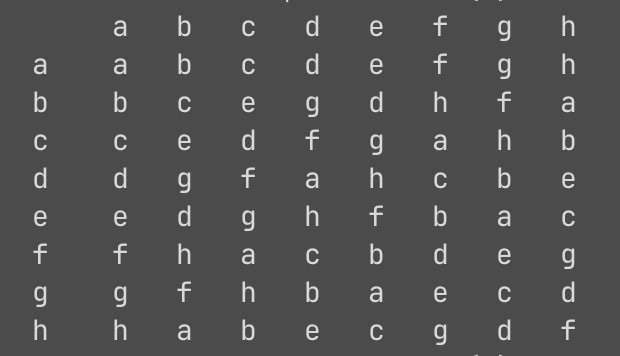
\includegraphics[width=\linewidth]{screenshots/add_table.jpg}
    \end{minipage}
    \hfill
    \begin{minipage}{0.48\textwidth}
        \centering
        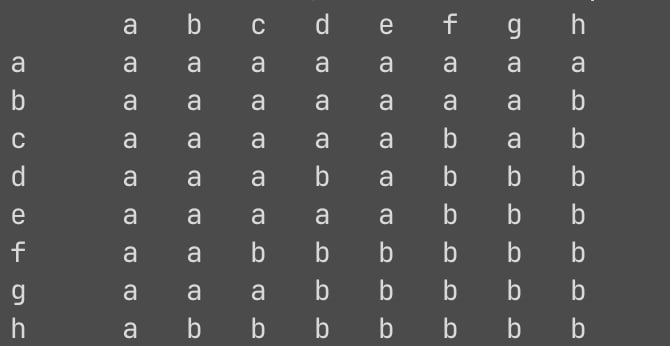
\includegraphics[width=\linewidth]{screenshots/carry_add_table.jpg}
    \end{minipage}
    \caption{Таблица сложения и таблица переносов для малой арифметики}
	\label{fig:add_table}
\end{figure}

\begin{figure}[h]
    \centering
    \begin{minipage}{0.48\textwidth}
        \centering
        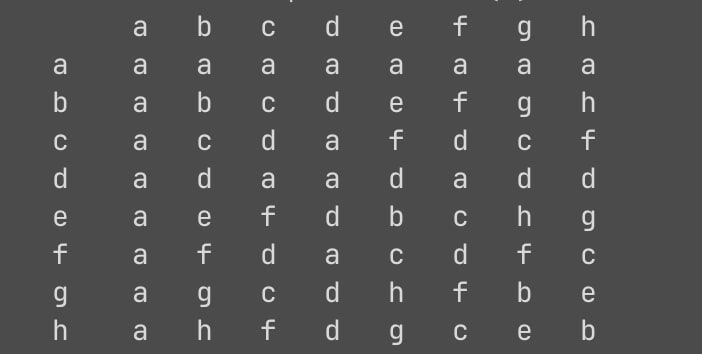
\includegraphics[width=\linewidth]{screenshots/mul_table.jpg}
    \end{minipage}
    \hfill
    \begin{minipage}{0.48\textwidth}
        \centering
        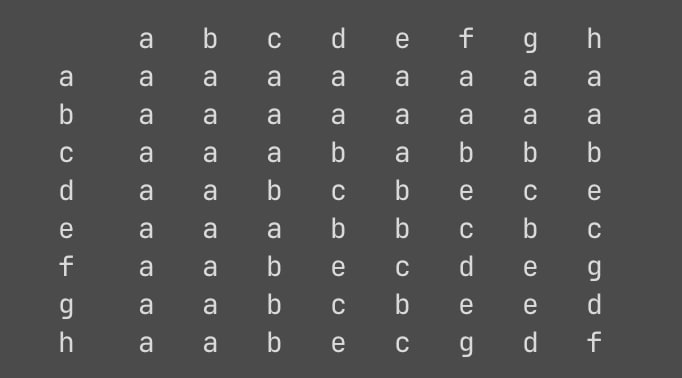
\includegraphics[width=\linewidth]{screenshots/carry_mul_table.jpg}
    \end{minipage}
    \caption{Таблица умножения и таблица переносов для малой арифметики}
	\label{fig:mul_table}
\end{figure}


\subsection{Примеры вычислений}

\begin{enumerate}
	\item $e + d = e + c + c = e + b + b + b + b = h$
	\item $g + c = g + b + b = f + b = h$
	\item $h + f = h + c + d = h + b + b + c + c = h + b + b + b + b + b + b = g$
	\item $d * c = d * (b + b) = d + d = a$
	\item $g * f = g * (g + b) = g * g + g = g * (b + d) = g + g + g * d = g + g + g*(b + e) = g + g + g + g*e = g + g + g + g * (c + b) = g + g + g + g + g * c = g + g + g + g + g * (b + b) = g + g + g + g + g + g = c + c + c = d + c = f$
\end{enumerate}